\chapter{Evaluation von Vergleichsprodukten}
Vergleichbare Produkte aufz�hlen
Vor- und Nachteile auflisten.
Fazit
\subsection{OpenNebula}
%TODO: Eigens Formulieren
OpenNebula ist eine Open Source Cloud L�sung, welche unter Verwendung verschiedener Industriestandards eine hochverf�gbare, skalierbare und h�chsteffiziente Virtualisierungplattform zur Verf�gung stellt.
So k�nnen virtuelle Systeme auf unterschiedlichen Hypervisioren und Storage-Systemen zentral administriert und �berwacht werden.
Beim Ausfall einer Komponente k�mmert sich OpenNebula um den Neustart der virtuellen Instanzen auf einem anderen Hostsystem.
Die Integration und Automatisierung einer vorhandenen heterogenen Landschaft ist somit ohne weitere Hardwareinvestitionen flexibel m�glich.
%Zitat: https://www.netways.de/produkte/opennebula/
Eine typische OpenNebula Installation sieht folgendermassen aus:
\begin{figure}[htbp]
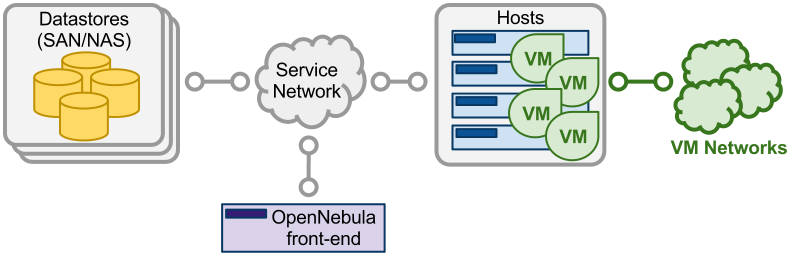
\includegraphics[scale=0.3]{../Bilder/one_high.png}
\caption{Typische OpenNebula Installation}
\label{fig: dasdasdasdas}
\end{figure}
Front-End: Steuert und fuhrt die OpenNebula Dienste aus. �
Schnittstelle fur den Cloud-Administrator. �
Konsolenbasiert oder graphisch (Sunstone Weboberfl�ache).
Hosts: Hosts mit installierter Hypervisor-Software.
Stellen die Ressourcen fur die Ausf � uhrung von virtuellen �
Maschinen.
Aktuell wird Xen, KVM und VMware als Hypervisor
unterstutzt, auch im Mischbetrieb. �
Datastores: Stellen die Basisimages (Betriebssysteminstallation,
Speicherplatz) der virtuellen Maschinen.
%Link: http://www.fbi.h-da.de/~a.schuette/Vorlesungen/Cloud-Computing/Skript/3_Cloud-Infrastrukturen/3_Cloud-Infrastrukturen.pdf
\subsection{VMware}

\subsection{IaaS}

